\section{Introduction}
\IEEEPARstart{A}{utonomous} warehouse transport must fit the geometry of racks, transfer gates, and loading pockets as well as the load capacity of vehicles. In confined aisles, changing orientation requires clearance for the complete tractor and payload. Recent studies in this journal improve tractor--trailer planning~\cite{xu2025,gatro2026}, generalized trailer trains~\cite{deniz2025}, motion representations~\cite{ddr2025}, and coordinated transport in dense environments~\cite{xu2024dense}. These advances also motivate a mechanical question: can a different connection make a previously obstructed maneuver possible?

A rigid vehicle carries its load in one body. A conventional articulated vehicle separates the tractor and payload, joined by a fixed drawbar. An inextensible cable permits an additional maneuver: the tractor can move toward the payload, create slack, and reposition while the payload remains stationary. Pulling resumes as the cable becomes taut. The material length stays fixed; the endpoint separation changes through cable bending. Figure~\ref{fig:warehouse} illustrates this operation near warehouse racks.

\begin{figure*}[!t]
\centering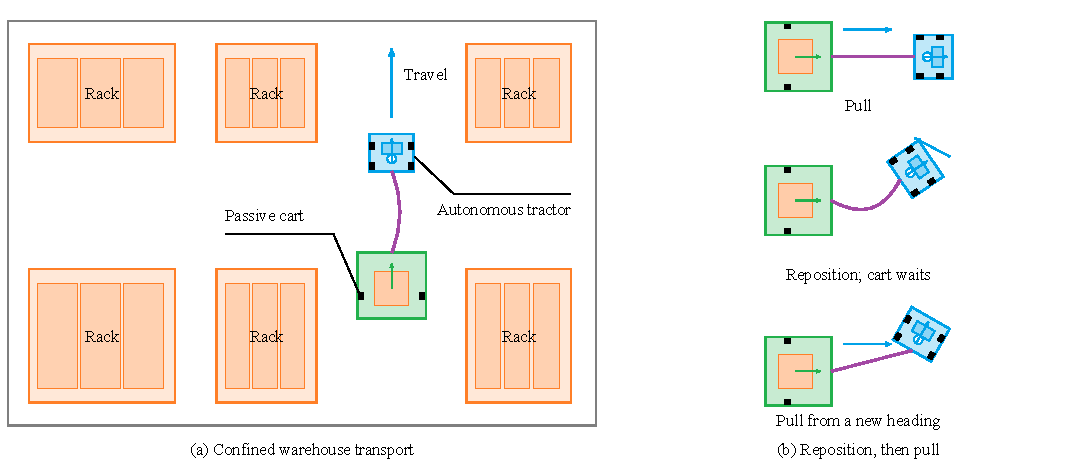
\includegraphics[width=\textwidth]{warehouse_concept.pdf}
\caption{Single-cart cable towing and tractor repositioning in a confined warehouse.}
\label{fig:warehouse}
\end{figure*}

The system comprises an autonomous car-like tractor and passive wheeled trailers, termed \emph{carts} hereafter. Propulsion, perception, planning, and tracking are concentrated in the tractor. A cable connection accommodates temporary formations and different cart outlines, while allowing the tractor to reposition independently of a waiting load. We study low-speed transport under a quasistatic mobility model: an unpulled cart stops immediately, and a pulled front hitch moves along the cable direction. These operating assumptions define the passive-cart class considered here. The resulting optimization-based planner prepares transport trajectories before task execution, starting from a feasible control sequence.

Cable towing has related precedents in leash-guided interaction~\cite{xiao2021}, collaborative quadruped towing~\cite{yang2022}, heterogeneous robot transport~\cite{xu2024cable}, and a quadruped towing a wheeled cart~\cite{zhang2026}. The present problem combines a curvature-bounded autonomous tractor, nonreversing passive carts, convex polygonal footprints, and repeated slack--taut transitions. Different payload outlines therefore change the feasible tractor motion.

Two questions organize the study. First, does cable coupling enable maneuvers excluded by a standard rigid drawbar with the same body geometry and length? Second, within the same cable system, which numerical strategy offers better trajectory quality, acceptance, and computation time? The contributions address these questions separately:
\begin{enumerate}
\item A six-state kinematic formulation combines Euler updates with a unilateral cable endpoint closure, supports convex polygonal footprints of arbitrary shape through optimization-based collision avoidance (OBCA)~\cite{obca2021}, and propagates recursively along serial carts. A geometric theorem identifies a rigid-coupling obstruction; corresponding cable trajectories are validated under the discrete model and geometric routing checks.
\item An optimization-based method for feasible-seed trajectory refinement combines relaxed initialization, feasible control restoration, replay-guided clearance reserves, and final recovery. Equivalent mode formulations and strategies adapted from published towing studies are compared under common models, maps, initial trajectories, and validation rules. Matched ablations isolate the numerical mechanisms.
\end{enumerate}
